\chapter{Digitalisierte Dokumente}
\label{chap:documents}
% Warum scannt man Dokumente

% Was für Dokumente werden gescannt

% 
Menschen erstellen Dokumente schon seit mehr als 4000 Jahren \parencite[13]{SmithDocumentCreationImage2014}. Dokumente, von Tontafeln (siehe \cref{fig:tablet})
bis hinzu rein digitalen Dokumenten, ermöglichen Kommunikation über zeitliche und ortliche Grenzen hinweg. 
Diese Technologie ist aus unserer modernen Kultur nicht mehr wegzudenken.  
Seit den 50er Jahren begann die Forschung im Bereich der Optischen Zeichenerkennung 
(engl. OCR)\autocite{DoermannHandbookdocumentimage2014}. OCR fand zuerst Einsatz in genau 
spezifizierten Problembereichen zum Beispiel die Erkennung von Druckbuchstaben einer Schreibmaschine. 
Je mehr Dokumente digitalisiert wurden, desto klarer wurde es das Dokumente mehr als 
eine Kette von Zeichen sind. 
Information können in Dokumenten über die Position der Zeichen und Skalierung von Zeichen vermittelt werden.
Zum anderen bestehen Dokumente aus Inhalten die semantische Bedeutung haben, aber nicht als Zeichenkette codiert werden können. 
%Eine Randnotiz
%\marginnote{Der Bezug dieses Satzes zum Text wird durch die Position verdeutlicht} setzt sich durch Formatierung und Position vom restlichen Text ab. 
\begin{marginfigure}
    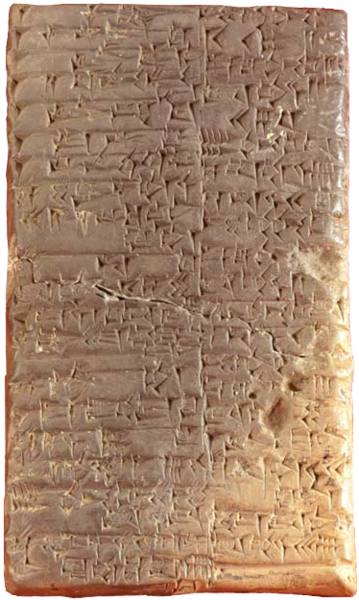
\includegraphics[width=\textwidth]{figures/img/359px-Cuneiform_script2.png}
    \caption{Königsliste (2047 Jahre v.Chr. \cite{DavidgeCuneiformscript2jpg})}
    \label{fig:tablet}
\end{marginfigure}


Wirtschaftsinteressen trieben die Entwicklungen von Dokumentenverarbeitungssystemen in einigen Bereichen sehr weit voran, wie 
zum Beipspiel bei der Verarbeitung von Geschäftsbriefen und Formularauswertung.
Eine Spezialisierung auf bestimmte Dokumentenklassen ist immer noch eine notwendigkeit angesichts der unzähligen, veränderbaren und nicht fest gelegten Gestaltungsmöglichkeiten für Dokumente \parencite[69]{BairdEvolutionDocumentImage2014}.

\section{Dokumente}
Typischerweise beschreiben wir ein Dokument als ein Papier mit einer Nachricht darauf. Diese Nachricht kann textueller Art sein, dass beudeutet Glyphen die in horizontalen oder vertikalen Lininen angeordnet sind (je nach Sprache)\parencite{BairdBriefHistoryDocuments2014}. Diese Textlininen sind dann meist in Textblöcken organisiert. Dokumente können auch grafische Inhalte haben. 
\qq{Warum sind alte Dokumente sind noch schwerer?}
Dokumente die mit modernen maschinellen Verfahren hergestellt sind einheitlicher in der Hinsicht, dass sie nicht nur einen einheitlichen Schriftsatz besitzen sondern auch alle anderen typografischen Parameter sind einheitlicher, auch Textlinien sind gerade und parallel.  

\section{Digitale Bibliotheken}
\qq{Was ist eine digitale Bibliothek?}
Immer mehr Bibliotheken und Archive arbeiten daran Sammlungen von Dokumenten zu digitalisieren und im Internet zur Verfügung zu stellen. 
Digitale Sammlungen sind dann nicht mehr an die Restriktionen von analogen Dokumenten gebunden und können deshalb auch seltene Dokumente oder Einzelstücke einer großen Menge von Nutzern züganglich machen.
Dies erleichtert besonders die Forschung an  historischen Dokumenten, da diese oft so wertvoll und fragil sind, dass die Lagerung und Nutzung der Originale strengen Auflagen unterliegen.

Die Digitalisierung ist aber nicht kostenfrei. Die Kosten belaufen sich bei Digitalisierungsprojekten in Deutschland auf etwa 10 bis 50 Cent pro Seite \parencite{OpitzWorkshopMassendigitalisierungsprojekteDeutschen2009}.
Die komplete Erfassung kann nochmals teurer sein, da die Erfassung von Strukturdaten zusätzliche Kosten verursacht. 
Im Digitalisierungsprojekt \emph{dünnhaupt digital} ist die Strukturdatenerfassung mit 40 Cent pro Seite der größte Ausgabenpunkt.
\cite{OpitzWorkshopMassendigitalisierungsprojekteDeutschen2009} bemerkt auch, dass die Volltextgenerierung mittels OCR nicht für eine sinnvolle Onlinenutzung nicht ausreichend ist. Erst die Erfassung von Seitenstrukturen erlaubt  ``einen gezielten Zugriff auf  logische Texteinheinten'' \parencite[372]{OpitzWorkshopMassendigitalisierungsprojekteDeutschen2009}.

Gescannnte Dokumente ohne eine symbolische Kodierung laufen Gefahr irrelevant zu werden,
da ihre Handhabung viel schlechter ist als die von ``purely digital information'' \parencite[10]{BairdDigitallibrariesdocument2003}.
 
\qq{Anforderungen an digitale Dokumente?}

\qq{Vereinheitlichung}

\section{Dokumentensegmetierung}



\section{Schritte in der Verarbeitung von Dokumentenbildern}
Die Dokumentensegmetierung ist ein Vorverarbeitungsschritt für weitere Schritte der Dokumentenverarbeitung.

Im Bereich der Bibliotheswissenschaften besteht ein großes Interesse an Klassifizierung von
Buchseiten zur besseren Erschließung.
\cite{McConnaugheyLabeledSegmentationPrinted2017} klassifizieren Buchseiten anhand von textbasierten Features in 4 Kategorien. 
Flow

\section{Auswahl und Beschreibung der Datensätze}
\textcite[985\psqq]{DoermannHandbookdocumentimage2014} listen 5 Aspekte die bei der Erstellung von Datensätzen zu beachten sind:
Auswahl der Daten
Datenbeschaffung
Ground Truth Definition
Ground Trouth Annotation
Speicherformat
Struktur und Organisation

\section{DIVA-HisDB}
Die DIVA \marginnote{\url{http://diuf.unifr.ch/main/diva/}} (Document, Image and Voice Analysis) Gruppe der Universität Fribourg hat im Kontext der Forschungsprojekte HisDoc und HisDoc 2.0 
das Datenset DIVA-HisDB. erstellt.
Die HisDoc-Projekte beschäftigen sich mit der automatischen Analyse von historischen Dokumenten und
wie man diese für Historiker nutzbar machen kann.

Für den Datensatz wurden Dokumente mit komplexen Layout aus der Virtuellen Manuskriptbibliothek der Schweiz (\url{http://www.e-codices.unifr.ch/en}) ausgesucht. Die Manuskripte enthalten neben dem Haupttext auch Randnotizen und Text-Dekorationen. Randnotizen befinden sich auch teilweise zwischen den Zeilen des Haupttexts.
 
DIVA-HisDB besteht aus 150 Dokumenten, aufgeteilt in Trainings-, Validierungs- und Testset (siehe \cref{table:hisdb_pages}. Hinzu kommen 30 Seiten die 
für die finale Wertung des Wettbewerbs ``ICDAR2017 Competition on Layout Analysis for Challenging Medieval Manuscripts'' verwendet wurden.

\begin{table}
    \caption{Aufteilung der Seiten des DIVA-HisDB-Datenssets}
    \label{table:hisdb_pages}
    \begin{tabular}{lccccc}
        {\bfseries Name} & {\bfseries Auflösung} & {\bfseries Training} & {\bfseries Validierung} & {\bfseries Test} & {\bfseries Test ICDAR 2017)}\\
        \csvreader[head to column names]{tables/diva_hisdb_specs.csv}{}%
        {\name&	\width \(\times\)\height & \train	&\validate	&\test	&\comp\\}
    \end{tabular}
\end{table}


Die Manuskripte wurden mit einer Auflösung von 600 dpi gescannt und sind im  JPEG-Format gespeichert. 
Die \cref{table:hisdbsamples} zeigt Beispiele aus den drei Datensätzen. 



Der Datensatz wurde semi-automatisch mit 3 Annotation (Haupttext, Kommentare, Dekorationen) versehen.
Diese Ground-Truth-Annotationen sind im PAGE-XML-Format und als ``pixel-label'' PNG-Bilder gespeichert.
Die \cref{fig:ground_truth} zeigt eine Beispielseite mit den zugehörgine Labels auf Pixelebene. 

\begin{figure*}
    \centering
    \caption{Hintergrund: weiss, Haupttext: blau, Kommentare: grün, Dekorationen: rot }
    \label{fig:ground_truth}
    \subfloat[Dokumentenbild]{%
        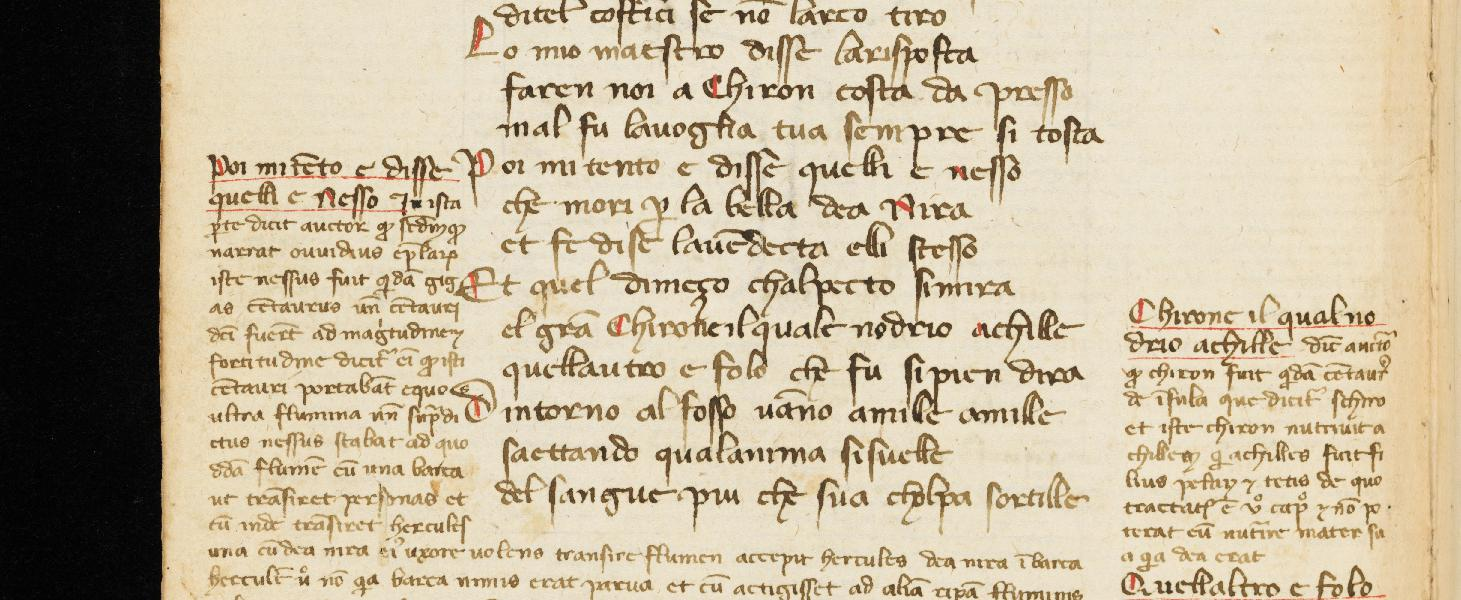
\includegraphics[width=0.5\textwidth]{figures/datasets/gt_example0.jpeg}
    }
    \subfloat[``pixel-label'']{%
        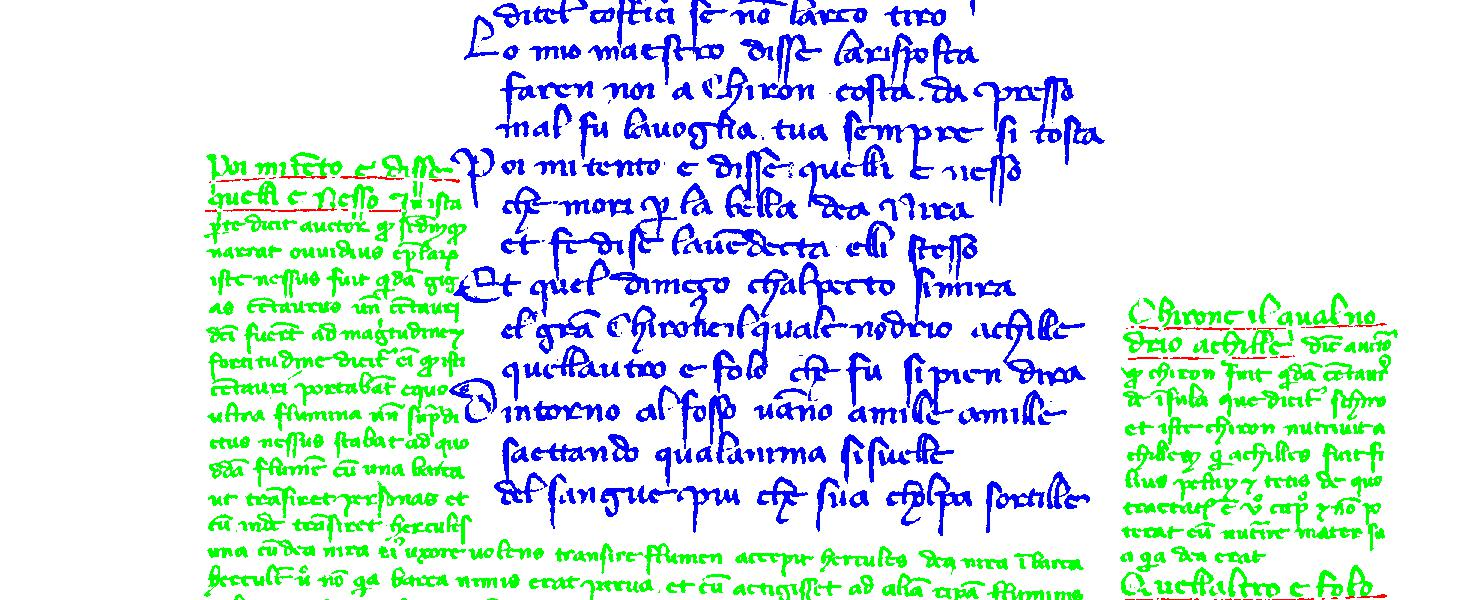
\includegraphics[width=0.5\textwidth]{figures/datasets/gt_example1.jpeg}
    }
\end{figure*}

Die Menge an Pixeln pro Klasse ist sehr unterschiedlich.
Die \cref{table:class_distribution} zeigt das in jedem Dokumentenset der Hintergrund deutlich überwiegt.

\begin{table}
    \caption{Verteilung der Klassen in Prozent\autocite[1362]{SimistiraICDAR2017CompetitionLayout2017}}
    \label{table:class_distribution}
    \begin{tabular}{lrrrr}
        {\bfseries Set} & {\bfseries Hintergrund} & {\bfseries Kommentar} & {\bfseries Dekoration} & {\bfseries Text}\\
        \csvreader[head to column names]{tables/diva_hisdb_class_distribution.csv}{}%
        {\set&	\background & \comments & \decoration & \text \\}
    \end{tabular}
\end{table}



\begin{table*}
    \begin{tabular}{llp{4cm}}
        \vspace{0.2cm}
        {\bfseries Seite} & {\bfseries Detailauschnitt} & {\bfseries Quelle } \\
        \vspace{0.5cm}
        
        \raisebox{-.5\height}{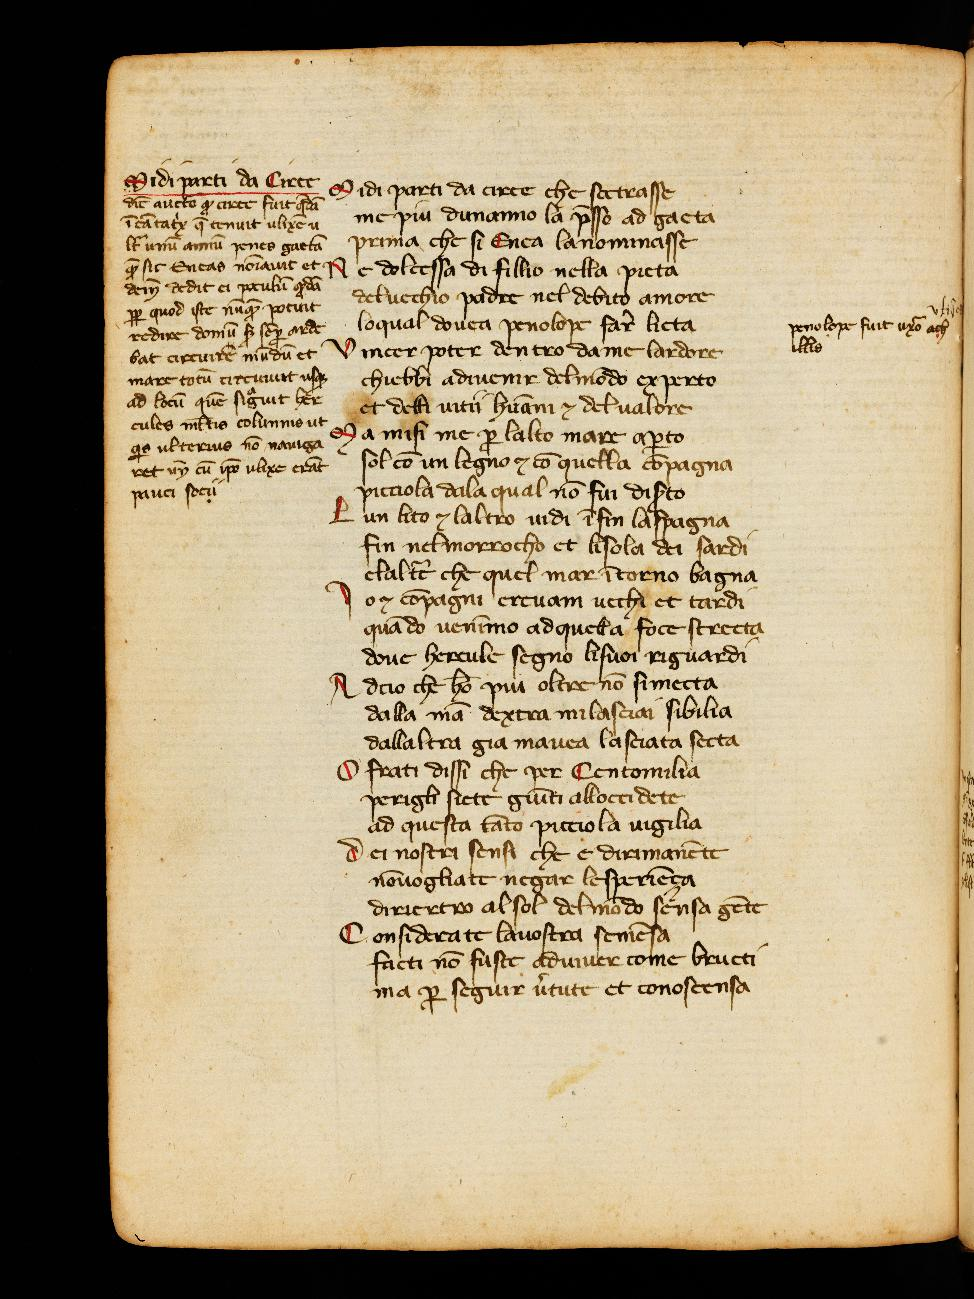
\includegraphics[height=4cm]{figures/datasets/HisDBSample0.jpeg}}
    &\raisebox{-.5\height}{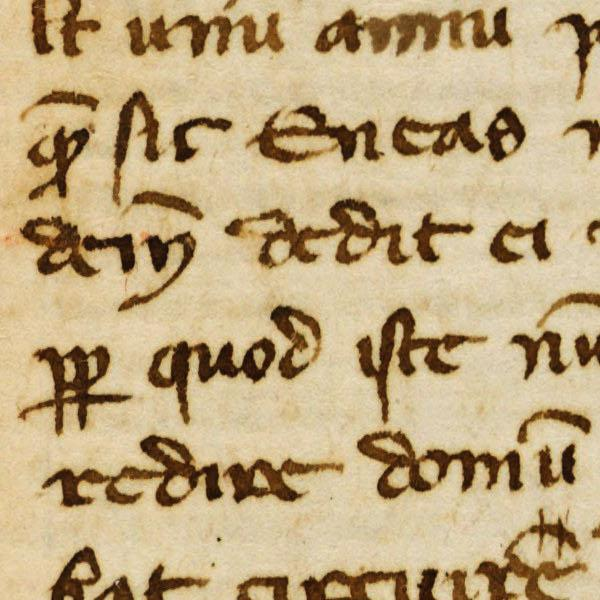
\includegraphics[height=4cm]{figures/datasets/HisDBSampleBox0.jpeg}}
     & \citefield{AlighieriColognyFondationMartin1300}{title}\\
     \vspace{0.5cm}  
     
    \raisebox{-.5\height}{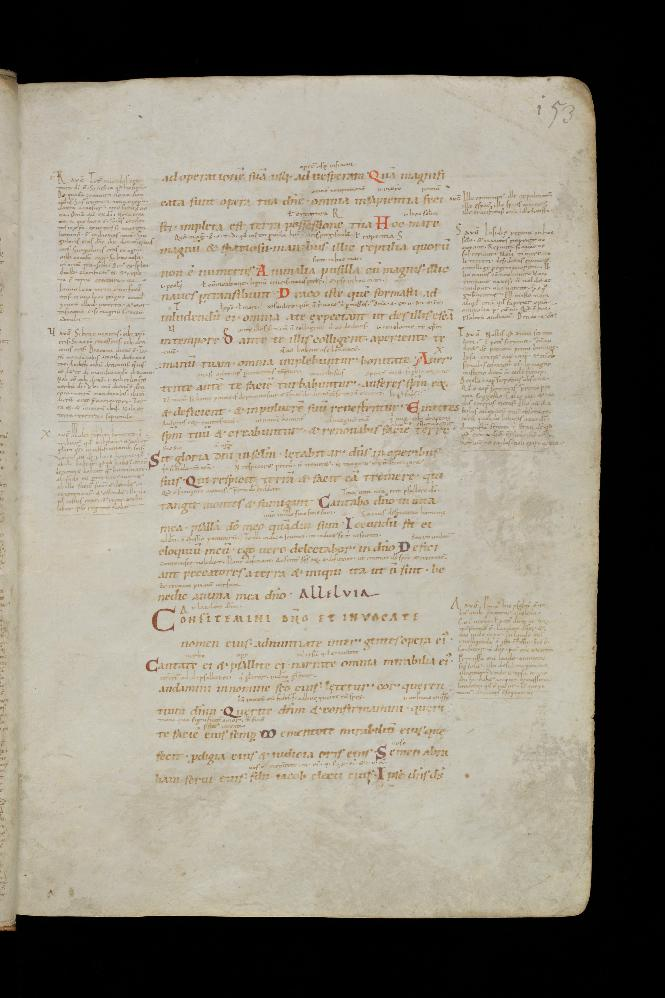
\includegraphics[height=4cm]{figures/datasets/HisDBSample2.jpeg}}
    & \raisebox{-.5\height}{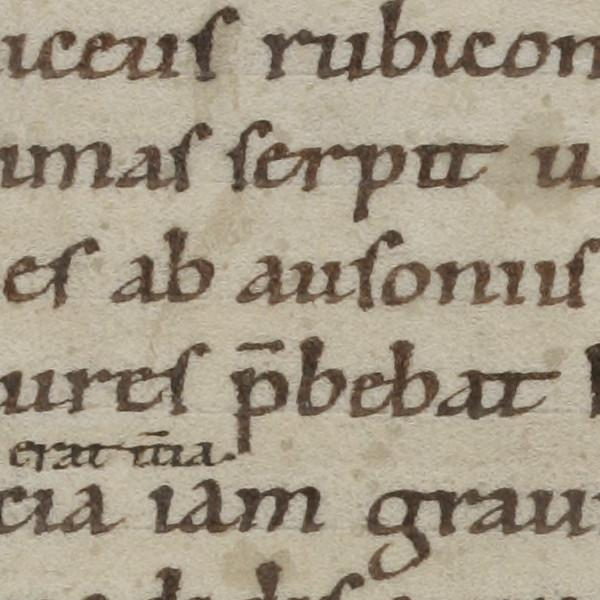
\includegraphics[height=4cm]{figures/datasets/HisDBSampleBox2.jpeg}}
    & \citefield{AmbrosiusStGallenStiftsbibliothek985}{title}\\
    \vspace{0.5cm}
    
     \raisebox{-.5\height}{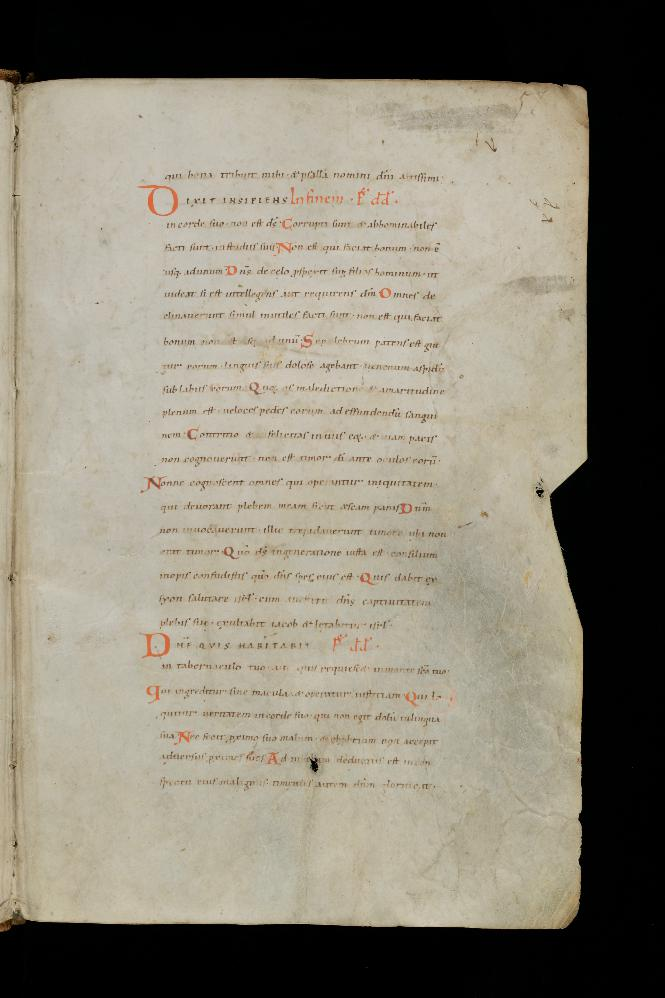
\includegraphics[height=4cm]{figures/datasets/HisDBSample1.jpeg}}
    &\raisebox{-.5\height}{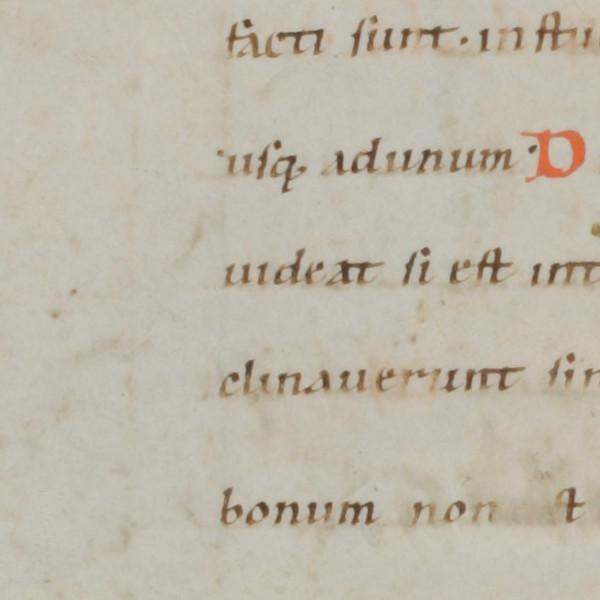
\includegraphics[height=4cm]{figures/datasets/HisDBSampleBox1.jpeg}}
     & \citefield{LucanusStGallenStiftsbibliothek1025}{title}\\
     \vspace{0.5cm} 

    \end{tabular}
    \caption{HisDB Beipsiele mit Detailauschnitt}
    \label{table:hisdbsamples}
\end{table*}

